\documentclass[tikz,border=2pt,11pt]{standalone}
\usetikzlibrary{arrows.meta}
\usetikzlibrary{backgrounds}
\usetikzlibrary{fit}
\usepackage{amsmath}
\usepackage{amssymb}
\usepackage{tikz}
\usepackage{xcolor}
\begin{document}
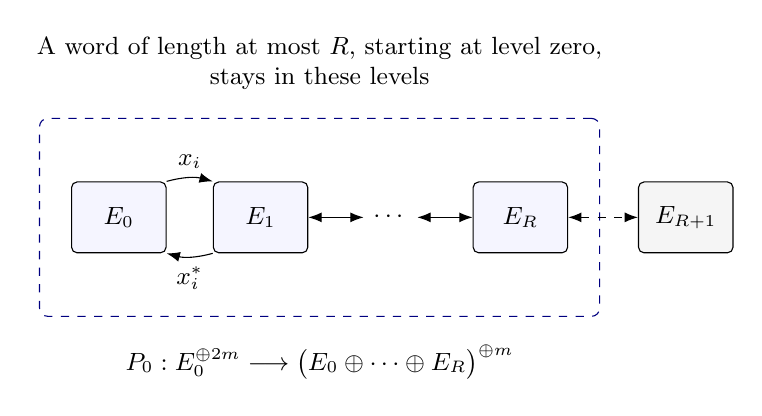
\begin{tikzpicture}[>=Latex, font=\small,
  level/.style={draw, rounded corners=2pt, minimum width=12mm,
                 minimum height=9mm, fill=blue!4}]
  \node[level] (e0) at (0,0) {$E_0$};
  \node[level] (e1) at (1.8,0) {$E_1$};
  \node (dots) at (3.45,0) {$\cdots$};
  \node[level] (er) at (5.1,0) {$E_R$};
  \node[level,fill=gray!8] (beyond) at (7.2,0) {$E_{R+1}$};
  \draw[->] (e0.north east) to[bend left=15] node[above] {$x_i$} (e1.north west);
  \draw[->] (e1.south west) to[bend left=15] node[below] {$x_i^*$} (e0.south east);
  \draw[<->] (e1) -- (dots);
  \draw[<->] (dots) -- (er);
  \draw[<->,dashed] (er) -- (beyond);
  \begin{scope}[on background layer]
    \node[draw=blue!50!black,dashed,rounded corners=3pt,
          inner xsep=4mm,inner ysep=8mm,fit=(e0)(er)] (window) {};
  \end{scope}
  \node[anchor=south,align=center] at (2.55,1.5)
    {A word of length at most $R$, starting at level zero,\\ stays in these levels};
  \node[anchor=north,align=center] at (2.55,-1.5)
    {$P_0:E_0^{\oplus 2m}\longrightarrow
       \bigl(E_0\oplus\cdots\oplus E_R\bigr)^{\oplus m}$};
\end{tikzpicture}
\end{document}
